\documentclass[12pt]{article}

\usepackage[utf8]{inputenc}
\usepackage{latexsym,amsfonts,amssymb,amsthm,amsmath}
\usepackage{tikz}
\usepackage{stanli}
\usetikzlibrary{shapes,calc,through,3d,patterns}
\usetikzlibrary{arrows.meta,decorations.pathreplacing,angles,quotes}
\usepackage{multicol}
\usepackage{geometry}
\usepackage{mathtools}
\usepackage{siunitx}
\usepackage{booktabs}

\setlength{\parindent}{0in}
\setlength{\oddsidemargin}{-0.25in}
\setlength{\textwidth}{7in}
\setlength{\textheight}{9.3in}
\setlength{\topmargin}{-1in}
\setlength{\headheight}{18pt}

\newcommand\blfootnote[1]{%
    \begingroup
    \renewcommand\thefootnote{}\footnote{#1}%
    \addtocounter{footnote}{-1}%
    \endgroup
}

\definecolor{darkred}{rgb}{0.6,0,0}

\newcommand{\bolddelta}{\boldsymbol\delta}
\newcommand{\boldxi}{\boldsymbol\xi}

\begin{document}

\noindent ME473 - Dynamic finite element analysis of structures\hfill EPFL\\
Stefano Burzio \hfill 2025\\
\vspace{0.3cm}

\hspace*{\fill}\textbf{\Large Problem set 2}\hspace*{\fill}

\hrulefill

\subsection*{Problem 1}
Consider the longitudinal vibrations of a free-free (not clamped at both ends) bar of length \( \ell \), with a constant cross-sectional area \( A \), constant Young's modulus \( E \), and constant material density \( \rho \). The longitudinal vibrations of the bar are governed by the one-dimensional wave equation:

\begin{equation*}
    \begin{cases}
        EA \, \partial^{2}_{xx} u_{1}(x, t) = \rho A \, \ddot{u}_1(x, t) \quad & \forall (x, t) \in ]0, \ell[ \times ]0, T[ \\
        EA \, \partial_{x} u_1(0, t) = 0 \quad                                 & \forall t \in ]0, T[                       \\
        EA \, \partial_{x} u_1(\ell, t) = 0 \quad                              & \forall t \in ]0, T[.
    \end{cases}
\end{equation*}
These equations are coupled with the initial conditions:
\begin{equation*}
    u_1(x, 0) = u_0(x), \quad \dot{u}_1(x, 0) = v_0(x), \quad \forall x \in ]0, \ell[.
\end{equation*}
Write the weak form and the semi-discrete weak form of the problem. Then approximate the first and second natural frequencies using a two-term Galerkin approximation based on the shape functions\footnote{Readers familiar with the finite element method will readily recognize that the chosen functions are linear combinations of the two basis functions of a one-dimensional two-node finite element. Furthermore, observe that \( h_1(0) \neq 0 \). What is the reason for this?}:
\begin{equation*}
    h_1(x) = 1, \quad h_2(x) = \frac{x}{\ell}.
\end{equation*}
Compare the relative error in the second fundamental frequency with the exact one, obtained by the analytical solution:

\begin{equation*}
    \omega_2^{\text{exact}} = \pi \sqrt{\frac{E}{\rho \ell^2}}.
\end{equation*}

Finally, provide a physical interpretation the first fundamental frequency.

\subsection*{Problem 2}
Write a \texttt{MATLAB} script to approximate the natural frequencies of a tapered bar of length $l=2\mbox{ m}$ which is fixed at the left end and spring-supported at the right end, as shown in the figure below.
\begin{center}
    \begin{tikzpicture}[scale=1]
        \point{a}{0}{0};
        \point{b}{0}{1.2};
        \point{c}{0}{-1.2};
        \point{d}{10}{0};

        \support {3}{a}[270];
        \support {3}{b}[270];
        \support {3}{c}[270];
        \support {5}{d}[90];

        % Draw the rectangle
        \filldraw[fill=gray!40, draw=black,thick] (0,-1.5) -- (10,-0.5) -- (10,0.5) -- (0,1.5) -- cycle;

        %axis
        \draw[-latex, ultra thin] (0,0) -- (11.7,0);
        \draw[ ultra thin] (0,-2) -- (0,2);
        \node at (12,0.5) {\(x\)};

        % length
        \draw[ultra thin] (10,0) -- (10, 2) ;
        \draw[latex-latex, ultra thin]  (0,1.7)  to node[sloped,midway,above] {$\ell$}(10,1.7) ;
        \draw[ultra thin]  (7,0.3) -- (8,-1) node[right]{$E,\rho$};

    \end{tikzpicture}
\end{center}
The governing equations are:
\begin{equation*}
    \begin{cases}
        \partial_{x}\big(EA(x) \partial_{x} u_{1}(x, t)\big) = \rho A(x) \, \ddot{u}_1(x, t) \quad & \forall (x, t) \in ]0, \ell[ \times ]0, T[ \\
        u_1(0, t) = 0 \quad                                                                        & \forall t \in ]0, T[                       \\
        EA(\ell) \, \partial_{x} u_1(\ell, t)+k u_1(\ell,t)= 0 \quad                               & \forall t \in ]0, T[.
    \end{cases}
\end{equation*}
The homogenous and isotropic bar is made of steel S235 and has Young's modulus $E = 210 \mbox{ GPa}$ and mass density $\rho=7850 \mbox{ kg/m}^{3}$.  The cross-sectional area of the bar follows a decreasing linear function:
\[
    A(x) = A_0 \big(1-\beta \frac{x}{\ell}\big)
\]
where \( A_0 = 150 \, \text{mm}^2 \) is the cross-section at \( x = 0 \), and \( \beta = 4/15 \) is the tapering coefficient. Moreover the spring characteristic constant has value $k=12 \mbox{ kN/m}$.

Apply the Galerkin method using two distinct sets of shape functions:
\begin{enumerate}
    \item \emph{Harmonic approximation:} a two-terms approximation based on harmonic functions.
    \item \emph{Polynomial approximation:} a two-terms approximation based on polynomial functions.
\end{enumerate}
For both approximations, compute the first two approximate natural frequencies. The units used in \texttt{MATLAB} are Newton (N), Pascal (Pa) and meter (m).

\blfootnote{Problem 1 is taken from [G] example 2.3.3}
\blfootnote{[G] Gmür, Dynamique des structures: analyse modale numérique. EPFL Press, 1997}
\end{document}